\chapter{Problem analysis \& Objectives}
\section{Analysis}
After confirming the data port on the back of the device did not provide enough control \footnote{The data port only allows input and output of audio, transfer of station memory when the radio is in a special mode and control of squelch level.}, it became clear that the only way to interface with the radio without opening up the case (and invalidating the warranty) was to utilise the serial line that connects the head and body of the radio.

Previous work on understanding the serial protocol between the body and head of the radio was undertaken and compiled by Ben Cooper \cite{ben_report}\cite{8800r_reverse}. This work helped to ascertain the basics of the serial communication. Ben Cooper's project was focused on developing software aimed to run on a Arduino microcontroller. He concludes that the severe complexity of sending, receiving and processing on a single thread was perhaps reason to consider other options.

Considering the application may need to be run in these remote shacks with limited power and Internet connectivity. The project will aim to be as power and memory efficient as possible, so that it can be run on low specification hardware. This gives the benefits of a lower cost. Additionally for this reason the application must be portable for at least the x86 and ARM architectures so that it is actually possible to run on a low spec machine. This will give the user as many options as possible, for example low power PCs such as the Raspberry Pi or to just control the radio straight from a laptop that has serial capabilities. Development of the project will also benefit as common laptop/desktop hardware can be used with the use of a USB \gls{ttl} dongle. These dongles are cheap and ubiquitous, often costing less than \pounds1 each. This gives a low barrier to entry as it is the only dedicated hardware required for most users.

\subsection{Protocol}
Most of the protocol was already reverse engineered by other authors such as Ben Cooper~\cite{ben_report}, these assumptions were confirmed using a digital oscilloscope by being able to decode both \gls{tx} and \gls{rx}. Figure~\ref{fig:circuit_diagram} shows a circuit diagram, the connectors at each end of the circuit are RJ25 ports (aka telephone jacks) with 6 active lines. In the order of left to right from the perspective of looking into the socket, the first 2 lines are for \gls{rx} and \gls{tx} of serial, ground, 9v power, power switch and the last line is for the microphone. The radio does not use the common RS232 standard\footnote{RS232 sends binary with -13V to represent a one bit and +13v for a 0 bit, allowing for easy knowledge of when the line is idle at 0V} instead it uses the older \gls{ttl} standard. In this case this means that an idle line is at 5V which represents a 1 bit and 0V representing 0 bit. The beginning of a transmission is marked with a single start bit, followed by 8 bits of data and then a single stop bit. There is no error checking through parity or otherwise. 

So to summarise the communication: 
\begin{itemize}
    \item 0-5V
    \item \gls{ttl} protocol
    \item 8 data bits with 1 stop bit
    \item The most significant bit is transferred first
    \item 19,200 baud rate
    \item Automatic shutoff after 80ms
\end{itemize}

\gls{tx} from the head to the body of the radio does two things. For analogue buttons it transmits the current state of those buttons and for digital encoders, such as the dials, it transmits the number of rotations since the last \gls{tx}. The packet of data that is sent consists of 13 bytes (mapped previously\cite{ben_report}). This could be utilised as a method to provide emulated input to the radio. Actions could be undertaken by the program to replicate any input that a human was capable of.

\begin{figure}
    \centering
    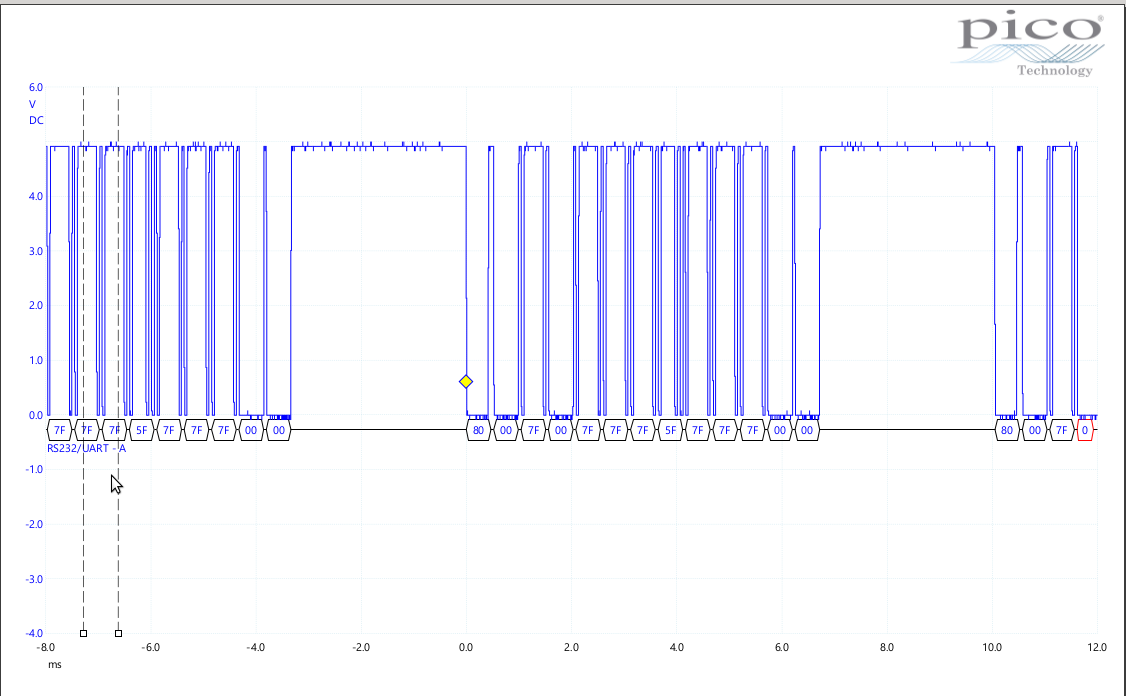
\includegraphics[width=1\textwidth]{img/controll_packet.png}
    \caption[Control packet]{A capture of control packets. The 2 long peeks are the begging and end of the middle packet}
    \label{fig:control_packet}
\end{figure}

\gls{rx} (from the body to the head) is a packet of 42 bytes. Each bit in the packet represents whether a segment of the screen should be illuminated or not, for example what frequency should be shown. The program can listen to this to learn the internal state of the radio. The state of the radio that is not represented on the screen will have to be discovered by navigating the menus and then reading the screen.

During the project there where some new observations made to the transmission protocol. The most significant bit (MSB) is transmitted first between the radio and head with a 20ms gap between both \gls{rx} and \gls{tx} packets. The head will transmit its \gls{tx} packets as soon as it is given power if the body is given the boot signal (setting the 5th line to low) but without receiving head packets it will shutdown after 80ms. The only indication of this boot failure is is a small audible click sound from the loudspeaker. 

\section{Aim \& Deliverables}
The scope of development efforts will be to create a way to control the body of the radio, with the aim to achieve as much functionality as possible (controllable by a computer). Communication to the head, for the purposes of using it as a generic control surface will remain out of scope. This non-critical feature would be at a high cost in time spent, when instead more important control features could be implemented. However work done that is in scope will be foundational to this feature if desired later. Dealing with the audio from the radio was also deemed out of scope, as the data-port of the back of the radio can already achieve this. Users can use a cable speaker line out and microphone line out from the back data port.

Below is a list of deliverables. Necessary functions were derived by asking a number of ``Customers'' what they would consider their minimum set of features (aka the planning game) and there expected difficulty. They are also in order of priority. Therefore this became the priority backlog.

\begin{itemize}
    \item Final report
    \item Software functions that have been deemed necessary for radio control:
        \subitem Frequency
        \subitem Push to talk
        \subitem Volume
        \subitem \gls{squelch}
        \subitem Power
        \subitem Powering on the radio
    \item Documentation
        \subitem Code documentation (\gls{doxygen})
        \subitem Schematic of prototype serial controller
\end{itemize}

Futures such as a more permanent printed circuit board and control of all functions of the radio were deemed not possible in the allotted semester of work\footnote{From \formatdate{30}{01}{2017} to \formatdate{08}{04}{2017}.}. Originally there was expressed intent on providing a patch to the open source Ham Radio Control Libraries, Hamlib\cite{hamlib}. The Initial report outline submitted reflected this. However after discussion of this intent on the developer mailing list it became clear that a multi-threaded application was unacceptable within the Hamlib codebase, due to concerns with portability and stability. Instead future work will likely include some sort of inter process communication through a socket.

\section{Security}
The envisioned scope of the project means that the software will not be networked in the modern sense of using IP communication. If the project did so there would be many security issues raised in how connections are handed, what kind of authentication is used and how will traffic be encrypted. Major operating systems manage access to serial communications often by requiring special privileges or groups. Therefore in this case, loss of access control can be prevented using just the default system configuration of most operating systems. The application will endeavour to not manipulate the system as much as is possible so as to minimise the attack surface given. Attention will be given to proper copying in memory and validation of incoming received serial communications to mitigate fuzzing based attacks.

Considerations must be made on who has physical access to the computer connected to the radio. As another user could plug the serial connection into their computer in order to interface with it, thereby forgoing the access control that was in place on the system. Users will also have to consult their local laws on whether it is legal for them to operate their radio remotely in their respective countries. 

\section{Process}
Due to the large potential scope of the project it was necessary to choose an agile methodology so that the large set of possible requirements could be better managed and prioritised. Therefore agile software development methodologies had to be constituted and chosen on their merit for the project. Methods considered were Scrum, \gls{xp} and \gls{fdd}. \gls{fdd} was quickly ruled out due to its major benefits only seen with larger teams that need to be able to produce regular status reports. For this project it was feared this would slow down the rate of development of features. Scrum was seen as less useful than \gls{xp} as it does not talk about the actual engineering steps to take in programming unlike \gls{xp}. Instead it focuses more on general management for a team. Therefore \gls{xp}\cite{extreme_programming} was chosen, however it still had to adapted for a single person project.

\gls{xp} guidelines for design can be summarised to the following\cite{xp}:
\begin{itemize}
    \item The Planning Game
    \item Small Releases (Iterations)
    \item System Metaphors
    \item Simple Design 	
\end{itemize}

\begin{figure}
    \centering
    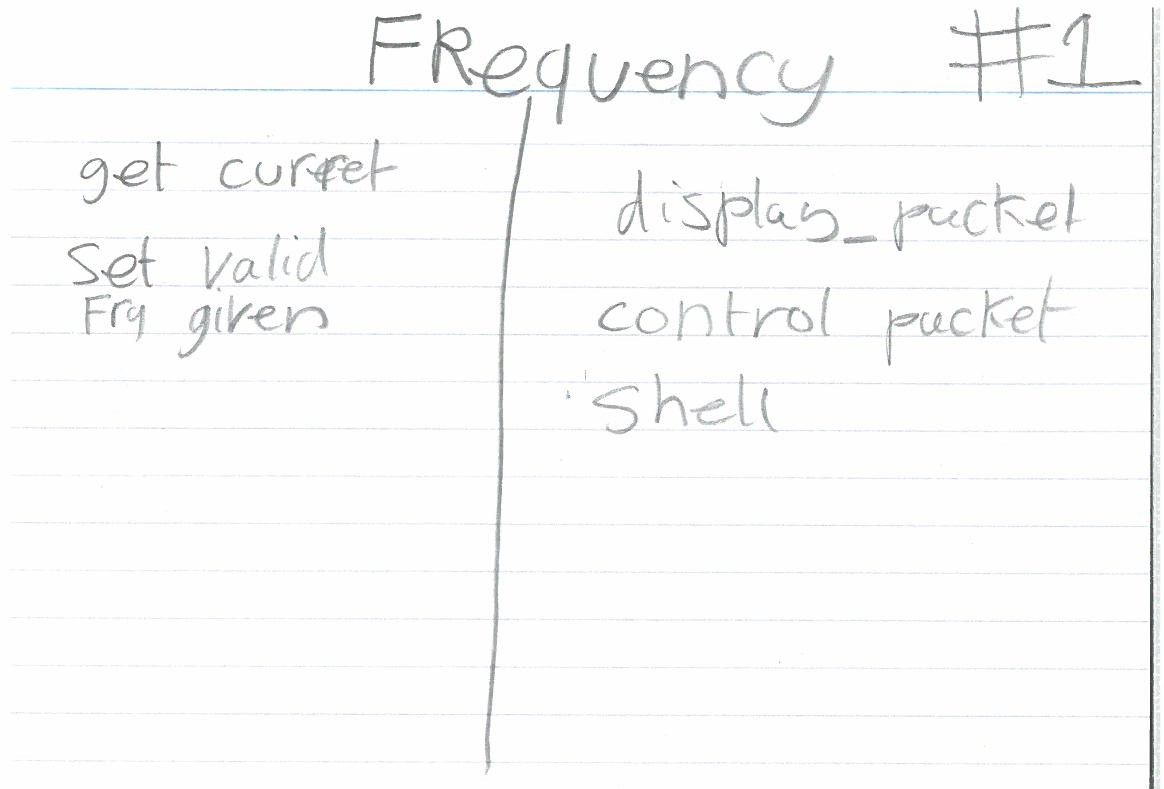
\includegraphics[width=0.5\textwidth]{img/crc_front}
    \caption[CRC front]{The front of the CRC cards contained on the left the required functions of the feature and what it will deal with on the right.}
    \label{fig:crc_front}
\end{figure}

\begin{figure}
    \centering
    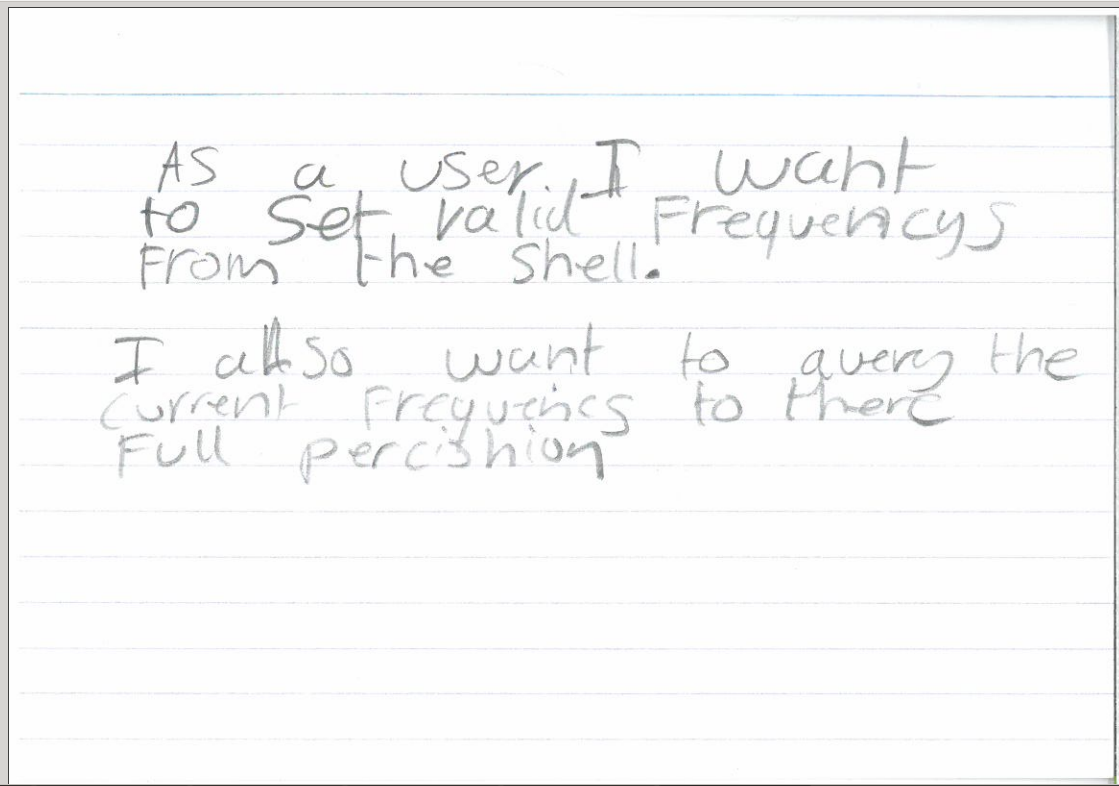
\includegraphics[width=0.5\textwidth]{img/crc_back}
    \caption[CRC back]{The back of the CRC cards contained the acceptance tests for the feature.}
    \label{fig:crc_back}
\end{figure}

The above points are very compatible for a lone developer project. The planning game was used with potential ``customers'' (Customers were any potential user of the radio i.e with the project supervisor), by requesting features to be prioritised. This was then used to produce and sort \gls{crc} cards (See figures ~\ref{fig:crc_front} and \ref{fig:crc_back} for the front and back of a \gls{crc} card respectively). Use of system metaphors was fairly common when discussing the project, this can been seen in this report with the ``head'' and ``body'' metaphors and standardisation of point of reference to serial communication with the \gls{rx}/\gls{tx} terms. Small releases at the end of each iteration were make allowing users give regular feedback. The initial design of the application was made to be just large enough to start development without the need for heavy refactoring later.

The actual development methods used in \gls{xp} will need to be modified in order to accommodate one developer. Thankfully adaption to a single developer as been discussed openly, including from the creator of \gls{xp}, Kent Beck in a number of mailing list discussions\cite{xpforone}\cite{lone_developer}.

The following sections will address the adaptations made:
\subsection*{Unit Tests}
The described use of unit tests do not need to be changed for the project. The test suite ``Google Tests''\cite{google_tests} was chosen despite the fact that this is implemented in C++, as it is often used to test C code and better support and features than native suites. Its test macros are familiar to programmers that have used suites such as JUnit etc. Unit tests were especially useful for the project as the real hardware was not always available for testing the radio was stored in a university lab that was shut on the evening, Fridays and weekends. 

\subsection*{Acceptance Tests}
Acceptance Tests are created on the back of \gls{crc} cards. A successful test is likely to be the ability for the user to preform said action on the real radio without any input from the developer. A passing acceptance test is the only verification of a completed feature.

\subsection*{Refactoring}
Refactoring should occur naturally throughout development as well as during the refactoring stage of creating a function with the \gls{rgf} method. Good use of unit tests will make refactoring easier as developers can make changes with confidence of not braking the system.

\subsection*{Pair Programming}
\gls{xp} has a heavy focus on pair programming. This project work is not permitted with other developers in order for a full assessment to take place of work done. Instead other methods that give some of the benefits of group collaboration such as``rubber ducking'' will be used. Rubber ducking is the process of talking out or explaining code to oneself in order to check that there are not better ways to do something. Throughout the project conversations with other students about the project, for example when walking up to campus was used to provide reflection. Questions from others asking why something was done in a particular way can often promote further analysis and better ideas.

\subsection*{Continuous Integration}
Git will be used as a VCS for the project using branches for new features before merging them, this was chosen over over VCS due to its better branching and mergeing as well as ability to still commit when disconnected from the Internet. Github will be used to host the central repository, due to its good user interface as well as its large popularity (meaning new user discovery is possible). A self hosted version of Jenkins\cite{jenkins} will used automatically test commits by running builds. Jenkins CI was chosen due to previous positive experiences with it as well as its high level of customisation owing to its large plugin library. 

\subsection*{Coding Standards}
The ``Linux kernel coding style''\cite{linux_coding_style} was chosen as it is a widely used standard that has a good rationale and format. To enforce a consistent style checking to was made in the text editor, as well as a step in continuous integration checks to look for style violations.

\subsection*{Iterations}
The project will run using two week iteration/release cycle. It is hoped that this will give enough time to plan, develop, and physically test the radio functions. In this time the current most needed feature from the priority backlog will be worked on. To do this a number of engineering tasks are made from the feature and placed as ``TODO'' items in the source code. This is the most appropriate place as tasks remain very visible until removed, unlike when tasks are recorded on a webpage elsewhere.  At the end of an iteration a release is tagged in git with a version number that conforms to the semantic versioning convention\cite{sem_ver}. Additionally a changelog is made on the developer blog. This means there are regular versions of the software that can be tested and reflections can be made about the progress of the project.
